% Homework Template
\documentclass[a4paper]{article}
\usepackage{ctex}
\usepackage{amsmath, amssymb, amsthm}
\usepackage{moreenum}
\usepackage{mathtools}
\usepackage{url}
\usepackage{bm}
\usepackage{enumitem}
\usepackage{graphicx}
\usepackage{subcaption}
\usepackage{booktabs} % toprule
\usepackage[mathcal]{eucal}
\usepackage[thehwcnt = 1]{iidef}


\usepackage{listings}
\usepackage{fontspec}
\usepackage{xcolor}

\usepackage{float}


\definecolor{codekeyword}{RGB}{171, 0, 216}
\definecolor{codetypename}{RGB}{29, 37, 251}
\definecolor{codevariable}{RGB}{10, 23, 126}
\definecolor{codestring}{RGB}{157, 0, 25}
\definecolor{codecomment}{RGB}{31, 129, 19}
\definecolor{codebackground}{RGB}{230 235 245}

\newfontfamily\cascadia[Ligatures=ResetAll]{Cascadia Code}
% \newfontfamily\codefont[Ligatures=ResetAll]{Cascadia Code}
% \newfontfamily\codefont[Ligatures=ResetAll]{Fira Code}[Contextuals={Alternate}]
% To enable ligature in listing, go check lstfiracode's github page and copy firacodestyle's settings.

\lstset{
    basicstyle          =   \small\cascadia,
    % ---
    tabsize             =   4,
    showstringspaces    =   false,
    numbers             =   left,
    numberstyle         =   \cascadia,
    % ---
    breaklines          =   true,
    captionpos          =   t,      
    % ---
    frame               =   l,
    flexiblecolumns,
    columns = fixed,
    % ---
    backgroundcolor     =   \color{codebackground},
}

\lstdefinestyle{Cppstyle}{
    identifierstyle     =   \color{codevariable},
    commentstyle        =   \color{codecomment},
    stringstyle         =   \color{codestring},
    keywordstyle        =   \color{codekeyword},
    keywordstyle        =   [2] \color{codetypename},
}


\setenumerate[1]{label=(\arabic{*})}
\setenumerate[2]{label=\arabic{*})}



\DeclareMathOperator{\arctanh}{arctanh}

\thecourseinstitute{清华大学电子工程系}
\thecoursename{\textbf{媒体与认知} \space 课堂2}
\theterm{2023-2024学年春季学期}
\hwname{作业}
\begin{document}
\courseheader
% 请在YOUR NAME处填写自己的姓名
\name{毕嘉仪}
\vspace{3mm}
\centerline{\textbf{\Large{理论部分}}}

\section{单选题(15分)}
% 请在?处填写答案
\subsection{\underline{B}}

\subsection{\underline{A}}

\subsection{\underline{B}}

\subsection{\underline{A}}

\subsection{\underline{B}}

\section{计算题(15 分)}
\subsection{设隐含层为$\mathbf{z}=\mathbf{W}^T\mathbf{x}+\mathbf{b}$,其中$\mathbf{x}\in R^{(m \times 1)}$,$\mathbf{z}\in R^{(n\times 1)}$,$\mathbf{W}\in R^{(m\times n)}$,$\mathbf{b} \in R^{(n\times 1)}$均为已知,其激活函数如下:
$$\mathbf{y}=\delta(\mathbf{z})=tanh(\mathbf{z})$$
tanh表示双曲正切函数。若训练过程中的目标函数为L,且已知L对$\mathbf{y}$的导数 $\frac{\partial L}{\partial \mathbf{y}}=[\frac{\partial L}{\partial y_1},\frac{\partial L}{\partial y_2},...,\frac{\partial L}{\partial y_n}]^T$和$\mathbf{y}=[y_1,y_2,...,y_n]^T$的值。}
\subsubsection{请使用$\mathbf{y}$表示出$\frac{\partial \mathbf{y}^T}{\partial \mathbf{z}}$, 这里的$\mathbf{y}^T$ 为行向量。}
\begin{proof}[解]
    
    \[\frac{\partial \boldsymbol{y}^\mathrm{T}}{\partial \boldsymbol{z}}_{n \times n} = 
    \begin{bmatrix}
        \frac{\partial y_1}{\partial z_1} & \dots & \frac{\partial y_n}{\partial z_1} \\
        \vdots & \ddots & \vdots \\
        \frac{\partial y_1}{\partial z_n} & \dots & \frac{\partial y_n}{\partial z_n} \\
    \end{bmatrix}\]
    当$i \neq j$, 易知 $\frac{\partial y_i}{\partial z_i} = 0$ \\
    当$i = j$, 
    \[\tanh^\prime z_i = 1 - \tanh ^2 z_i\]
    \[ z_i = \arctanh  y_i\]
    \[\therefore \tanh^\prime z_i = 1 - y_i^2\]
    \[\therefore \frac{\partial \boldsymbol y^\mathrm{T}}{\partial \boldsymbol z}_{n \times n} = \diag (1 - y_i^2) = 
    \begin{bmatrix}
        1 - y_1^2 & & & \\
         & 1 - y_2^2 & & \\
         & & \ddots & \\
         & & & 1 - y_n^2 \\
    \end{bmatrix}\]
\end{proof}

\subsubsection{请使用$\mathbf{y}$和$\frac{\partial L}{\partial \mathbf{y}}$表示$\frac{\partial L}{\partial \mathbf{x}}$,$\frac{\partial L}{\partial \mathbf{W}}$,$\frac{\partial L}{\partial \mathbf{b}}$。}
提示:$\frac{\partial L}{\partial \mathbf{x}}$,$\frac{\partial L}{\partial \mathbf{W}}$,$\frac{\partial L}{\partial \mathbf{b}}$与x,W,b具有相同维度。
\begin{proof}[解]
    对$\frac{\partial L}{\partial \boldsymbol x}$, 由链式法则:
    \[\frac{\partial L}{\partial \boldsymbol x}_{m \times 1} = \frac{\partial \boldsymbol z^{\mathrm T}}{\partial \boldsymbol x}_{m \times n} \frac{\partial \boldsymbol y^{\mathrm{T}}}{\partial \boldsymbol z}_{n \times n} \frac{\partial L}{\partial \boldsymbol y}_{n \times 1} = W \dot \diag (1 - y_i^2)\frac{\partial L}{\partial \boldsymbol y}\]
    对于$\frac{\partial L}{\partial W}$,先计算
    \[\frac{\partial \boldsymbol z_i}{\partial W}_{m \times n} = 
    \begin{bmatrix}
        \frac{\partial z_i}{\partial W_{11}} & \dots & \frac{\partial z_i}{\partial W_{1n}} \\
        \vdots & \ddots & \vdots \\
        \frac{\partial z_i}{\partial W_{m1}} & \dots & \frac{\partial z_i}{\partial W_{mn}} \\
    \end{bmatrix} = \begin{bmatrix}
        0 & \dots & \frac{\partial z_i}{\partial W_{1i}} & \dots & 0 \\
        \vdots & & \vdots & & \vdots \\
        0 & \dots & \frac{\partial z_i}{\partial W_{mi}} & \dots & 0 \\
    \end{bmatrix} \]
    \[ = \begin{bmatrix}
        & & x_1 & & \\
        & & \vdots & & \\
        & & x_m & & \\
    \end{bmatrix} = \begin{bmatrix}
        0 & \dots & \boldsymbol x & \dots & 0 \\
    \end{bmatrix}\]
    \begin{multline*}
        \therefore \frac{\partial L}{\partial W}_{m \times n} = \left(
        \frac{\partial \boldsymbol z_1}{\partial W}_{m \times n} \frac{\partial \boldsymbol y^{\mathrm{t}}}{\partial \boldsymbol z}_{n \times n} \frac{\partial L}{\partial \boldsymbol y}_{n \times 1}, \frac{\partial \boldsymbol z_2}{\partial W} \frac{\partial \boldsymbol y^{\mathrm{T}}}{\partial \boldsymbol z} \frac{\partial L}{\partial \boldsymbol y}, \dots, \frac{\partial \boldsymbol z_n}{\partial W} \frac{\partial \boldsymbol y^{\mathrm{T}}}{\partial \boldsymbol z} \frac{\partial L}{\partial \boldsymbol y}\right)_{m \times n} \\
        = \left(\boldsymbol x \diag(1 - y_i^2)\frac{\partial L}{\partial \boldsymbol y}, \dots, \boldsymbol x \diag(1 - y_i^2)\frac{\partial L}{\partial \boldsymbol y}\right) \\
    \end{multline*}
    对于$\frac{\partial L}{\partial \boldsymbol b}$,先计算
    \[\frac{\partial \boldsymbol z^{\mathrm{T}}}{\partial \boldsymbol b}_{n \times n} = \begin{bmatrix}
        \frac{\partial z_1}{\partial b_1} & \dots & \frac{\partial z_n}{\partial b_1} \\
        \vdots & \ddots & \vdots \\
        \frac{\partial z_1}{\partial b_n} & \dots & \frac{\partial z_n}{\partial z_n}\\
    \end{bmatrix} = I_n\]
    \[\therefore \frac{\partial L}{\partial \boldsymbol b}_{n \times 1} = \frac{\partial \boldsymbol z^{\mathrm{T}}}{\partial \boldsymbol b}_{n \times n} \frac{\partial \boldsymbol y^{\mathrm{T}}}{\partial \boldsymbol z}_{n \times n} \frac{\partial L}{\partial \boldsymbol y}_{n \times 1} = \diag(1 - y_i^2) \frac{\partial L}{\partial \boldsymbol y}\]
\end{proof}

\vspace{6mm}

\centerline{\textbf{\Large{编程部分}}}

\vspace{3mm}

\section{编程作业报告}
% 请在此处完成编程作业报告
\begin{enumerate}
    \item 使用默认配置对模型进行训练和测试。
    \begin{enumerate}
        \item 训练模型:
        
        input:
        \lstinputlisting{MyFile/1_1_in.txt}

        output:
        \lstinputlisting{MyFile/1_1_out.txt}

        \begin{figure}[H]
            \centering
            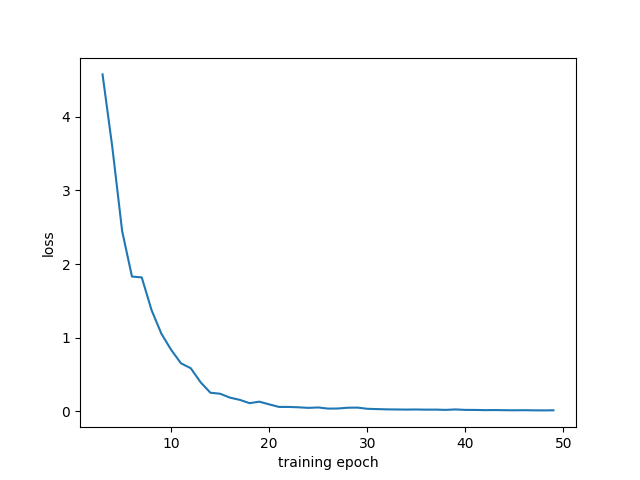
\includegraphics[width=0.65\linewidth]{MyFile/img/1_1.png}
            \caption{}
        \end{figure}


        \item 测试模型:
        
        input:
        \lstinputlisting{MyFile/1_2_in.txt}

        output:
        \lstinputlisting{MyFile/1_2_out.txt}


    \end{enumerate}
    \item 调整优化器为 Adam 优化器,修改其他参数,观察网络训练、验证和测试的性能。
    \begin{enumerate}
        \item 训练模型
        
        input:
        \lstinputlisting{MyFile/2_1_in.txt}

        output:
        \lstinputlisting{MyFile/2_1_out.txt}
        
        \begin{figure}[H]
            \centering
            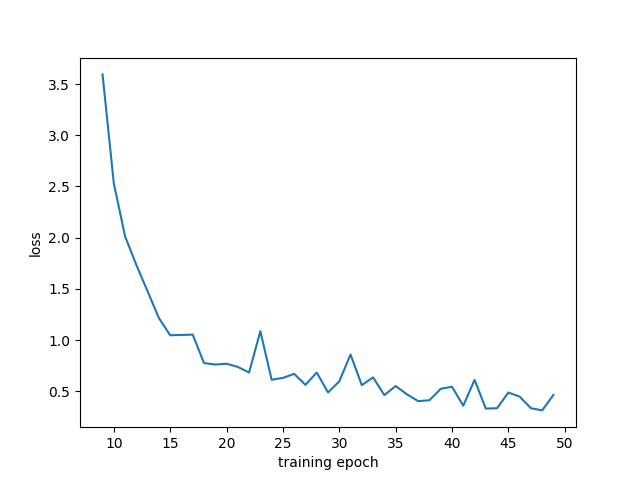
\includegraphics[width=0.7\linewidth]{MyFile/img/2_1.png}
            \caption{}
        \end{figure}

        \item 测试模型
        
        input:
        \lstinputlisting{MyFile/2_2_in.txt}

        output:
        \lstinputlisting{MyFile/2_2_out.txt}

    \end{enumerate}
    \item 选择效果最好的模型,对新的图像进行识别。
    \begin{enumerate}
        \item 选择模型:
        
        经过一些尝试,以下模型预测准确值为$85.5\%$,遂选取该模型进行预测:

        input:
        \lstinputlisting{MyFile/3_1_in.txt}

        output:
        \lstinputlisting{MyFile/3_1_out.txt}
        
        \begin{figure}[H]
            \centering
            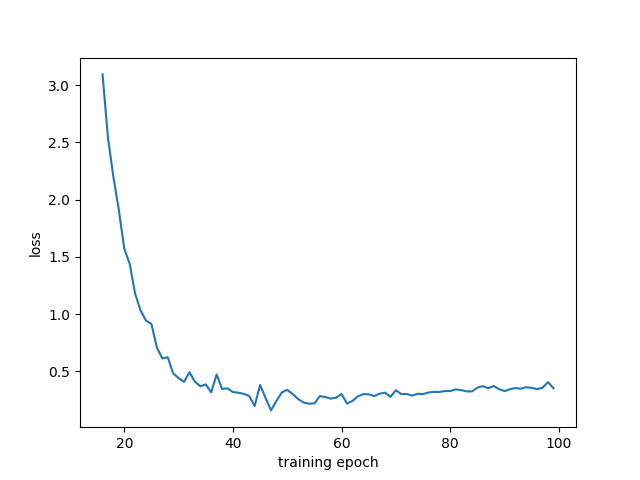
\includegraphics[width=0.7\linewidth]{MyFile/img/ADAM_opt_trial_lr1e-3_momentum15_epoch100.png}
            \caption{}
        \end{figure}

        input:
        \lstinputlisting{MyFile/3_2_in.txt}

        output:
        \lstinputlisting{MyFile/3_2_out.txt}

        \item 进行预测:
        
        input respectively:
        \lstinputlisting{MyFile/3_3_in.txt}
        
        prediction results:

        \begin{figure}[H]
	        \centering
	        \begin{subfigure}[b]{.3\linewidth}
	            
\includegraphics[width=\linewidth]{HW1-release/data/character_classification/new_images/1_W.jpg}
            \subcaption{pred: W}
	        \end{subfigure}
	        \hfill
	        \begin{subfigure}[b]{.05\linewidth}
	            
\includegraphics[width=\linewidth]{HW1-release/data/character_classification/new_images/2_I.jpg}
            \subcaption{pred: I}
	        \end{subfigure}
	        \hfill
	        \begin{subfigure}[b]{.17\linewidth}
	            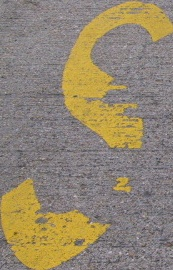
\includegraphics[width=\linewidth]{HW1-release/data/character_classification/new_images/3_S.jpg}
            \subcaption{pred: S}
	        \end{subfigure}
            \hfill
	        \begin{subfigure}[b]{.1\linewidth}
	            
\includegraphics[width=\linewidth]{HW1-release/data/character_classification/new_images/4_H.jpg}
            \subcaption{pred: H}
	        \end{subfigure}

            \hfill
            \begin{subfigure}[b]{.17\linewidth}
	            
\includegraphics[width=\linewidth]{HW1-release/data/character_classification/new_images/5_Y.jpg}
            \subcaption{pred: Y}
	        \end{subfigure}
	        \hfill
	        \begin{subfigure}[b]{.22\linewidth}
	            
\includegraphics[width=\linewidth]{HW1-release/data/character_classification/new_images/6_O.jpg}
            \subcaption{pred: O}
	        \end{subfigure}
	        \hfill
	        \begin{subfigure}[b]{.22\linewidth}
	            
\includegraphics[width=\linewidth]{HW1-release/data/character_classification/new_images/7_U.jpg}
            \subcaption{pred: U}
	        \end{subfigure}
            \hfill

            \hfill
	        \begin{subfigure}[b]{.22\linewidth}
	            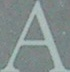
\includegraphics[width=\linewidth]{HW1-release/data/character_classification/new_images/8_A.jpg}
            \subcaption{pred: A}
	        \end{subfigure}
            \hfill
            \hfill

            \begin{subfigure}[b]{.22\linewidth}
	            
\includegraphics[width=\linewidth]{HW1-release/data/character_classification/new_images/9_N.jpg}
            \subcaption{pred: N}
	        \end{subfigure}
	        \hfill
	        \begin{subfigure}[b]{.07\linewidth}
	            
\includegraphics[width=\linewidth]{HW1-release/data/character_classification/new_images/10_I.jpg}
            \subcaption{pred: M}
	        \end{subfigure}
	        \hfill
	        \begin{subfigure}[b]{.22\linewidth}
	            
\includegraphics[width=\linewidth]{HW1-release/data/character_classification/new_images/11_C.jpg}
            \subcaption{pred: E}
	        \end{subfigure}
            \hfill
	        \begin{subfigure}[b]{.22\linewidth}
	            
\includegraphics[width=\linewidth]{HW1-release/data/character_classification/new_images/12_E.jpg}
            \subcaption{pred: E}
	        \end{subfigure}

            \hfill
            \begin{subfigure}[b]{.3\linewidth}
	            
\includegraphics[width=\linewidth]{HW1-release/data/character_classification/new_images/13_D.jpg}
            \subcaption{pred: D}
	        \end{subfigure}
	        \hfill
	        \begin{subfigure}[b]{.22\linewidth}
	            
\includegraphics[width=\linewidth]{HW1-release/data/character_classification/new_images/14_A.jpg}
            \subcaption{pred: A}
	        \end{subfigure}
	        \hfill
	        \begin{subfigure}[b]{.22\linewidth}
	            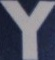
\includegraphics[width=\linewidth]{HW1-release/data/character_classification/new_images/15_Y.jpg}
            \subcaption{pred: Y}
	        \end{subfigure}
            \hfill
	    \end{figure}


    \end{enumerate}
    \item 遇到的问题及解决方法。
    \begin{enumerate}
        \item 在将样本图片转化为一维向量而使用tensor.flatten(input, start\_dim=0)函数时,没有注意到tensor变量imgs的第$0$维是batch\_size,导致后续计算tensor维数错误。因为一开始就对tensor.flatten(input, start\_dim=0)用法不确定,多留意了一下,侥幸发现了这个问题。
        \item 使用tensor.sum()时总是搞不清楚叠加的维度究竟是哪一维。借助浏览器的力量解决了这一问题。
        \item 没有注意到opt的hsize参数default$=32$,而模型训练的时候用的是$64$;进行预测时又没有指定hsize,导致tensor维度不对应。在重新查看了run command之后发现了这个小错。
    \end{enumerate}
    \item 建议:也许可以多介绍一下目录里各个类型的文件都是用来做什么的?第一次搭模型,很多文件类型都没见过,不知道它们有什么用。
\end{enumerate}

\end{document}